\section{ICON Overview}
\label{sec:approach}

\begin{figure}
	\centering
		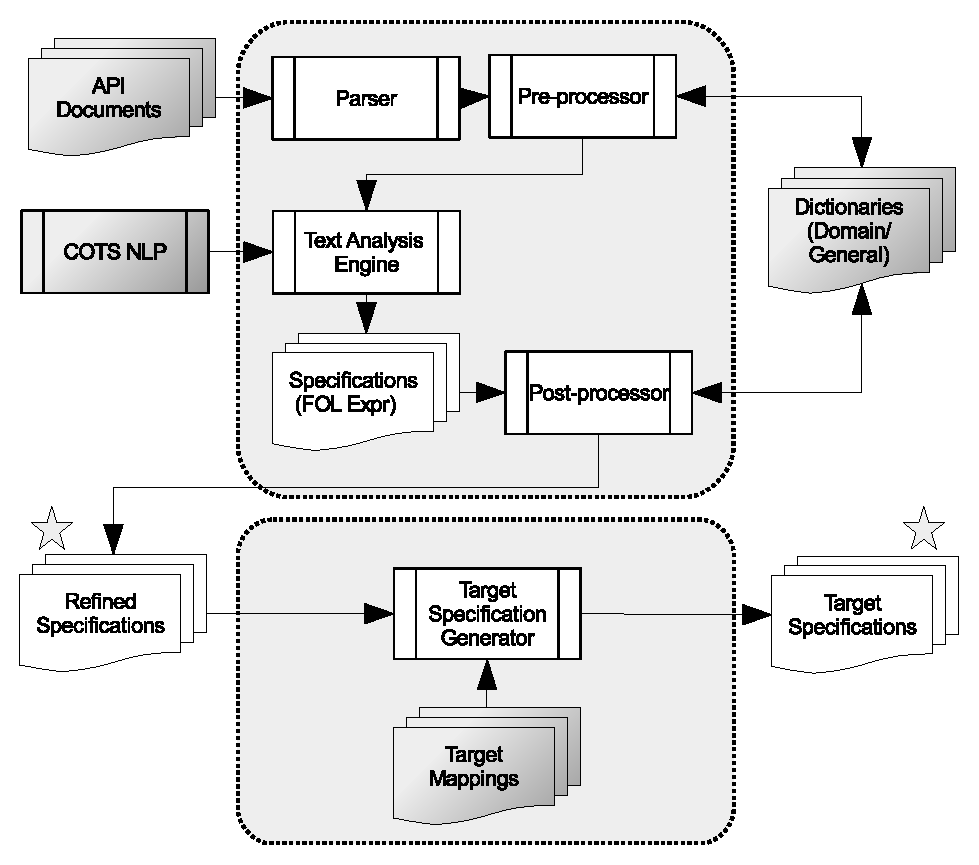
\includegraphics[scale=0.45]{approach.eps}
	\caption{Overview of the \tool\ approach}
	\label{fig:approachOverview}
\end{figure}

We next present our approach for inferring temporal constraints
from the method descriptions in API Documents.
Figure~\ref{fig:approachOverview} gives an overview of the \tool\ approach.
\tool\ consists of six major components: a preprocessor, a candidate identifier, a text-analysis engine, a semantic graph generator, constraint extractor, and a type analyzer.
Additionally, there is an optional model trainer component and external NLP parser component.


First, the preprocessor accepts API documents and preprocesses the sentences in the method description.
%such as annotating sentence boundaries and reducing lexical tokens.
Next, an NLP parser annotates the syntax and semantics of preprocessed sentences.
The annotated sentences are accepted by candidate identifier component to classify temporal constraint sentences,
using the model trained by the model trainer component.
The text-analysis engine further transforms the identified constraint sentences into the first-order-logic (FOL) representation.
Finally, the constraint extractor leverages the semantic graphs to infer temporal constraints from the FOL representation of a sentence.
The type analyzer component infers temporal constraints encoded in the type system of a language by analyzing the API methods parameter and return types.
We next describe each component in detail.


\subsection{Preprocessor}
\label{sub:prep}

The preprocessor accepts the API documents and extracts method descriptions.
In particular, the preprocessor extracts the following fields from the method descriptions: 
1) Summary of the API method,
2) Summary and type information of parameters of the API method, 
3) Summary and type information of return values of the method, and
4) Summary and type information of exceptions thrown (or errors returned) by the methods.

This step is required to extract the desired descriptive text from the API documents.
Different API documents may have different styles of presenting information to developers.
This difference in style may also include the difference in the level of the details presented to developers.
\tool\ relies only on basic fields that are generally available for API methods across different presentation styles. 

After extracting desired information, the natural language text is further preprocessed to be analyzed by subsequent components.
The preprocessing steps are required to increase the accuracy of core NLP techniques (described in Section~\ref{sub:CoreNLPback}) that are used in the subsequent phases of the \tool\ approach.
The preprocessor first employs the heuristics listed under lexical token reduction, as introduced in Section~\ref{sub:SENLPback}.

%Although the previous techniques and heuristics significantly lower the number of lexical tokens in a sentence,
%some sentences may still contain a considerable number of lexical tokens to overwhelm the POS tagger.
%To address this issue, we propose a new heuristic (\textit{`Frequent Phrases Reduction'})
%to further reduce the number of lexical tokens in a sentence by annotating frequent phrases as a single lexical unit.
%
%In particular, we use n-gram~\cite{brown1992class} based approach to achieve this reduction. 
%In the fields of computational linguistics, an n-gram is a contiguous sequence of n words from a given text.
%In statistical NLP and information theory, n-gram has been shown to be effective in computing the probability of occurrence of next word given a sequence of words.
%However, for \tool\ we use n-grams that always occur together in a given body of text.
%
%
%To achieve \textit{frequent phrases reduction}, we first calculate the most frequently occurring n-grams in the text body. 
%In particular, we are interested in the n-grams of length four or greater to achieve a reasonable reduction.
%We chose four as a threshold for n-grams because we observed that bigrams (size two) and trigrams (size three) frequently resulted in change of semantics
%of the sentence in comparison to n-grams of size four or grater.
%We then prune the list of n-grams based on a subsumption. 
%We consider an n-gram of length k ($n_k$) to subsume n-gram of length k-1 ($n_{k-1}$) iff $n_{k-1}$ is a substring of ($n_k$) and the frequency of occurrence of $n_{k-1}$ equals frequency of occurrence of $n_{k}$.
%Finally, we rank the list of n-grams based on the frequency of their occurrence in the text, and select top-k n-grams for reduction.
%For instance, \textit{Amazon Simple Storage Service}, \textit{an I/O Error Occurs}, and \textit{end of the stream} are the examples of such n-grams detected by \tool.


%\textbf{Prototype Implementation.}
%Currently our prototype implementation works with online \amazon\ and JDK API. 
%However, almost all of the developer documents are provided online as structured webpages.
%Thus, current prototype implementation of preprocessor can be easily extended to extract the desired information from any API developer documents.  
%
%Additionally, in current implementation we have manually built the dictionaries for preprocessing using the glossary of terms collected from the websites pertaining to REST and Java API.
%We further leveraged the HTML style information in \amazon\ to look for words that were highlighted in code like format. We further leveraged WordNet to maintain a static lookup table of shorthand words to aid named entity handling and abbreviation handling. 
% 
%Finally, to achieve n-gram reduction we used Apache Lucene~\cite{lucene}.
%Apache Lucene is a high-performance, full-featured text-search-engine library written entirely in Java,
%facilitating scalable cross-platform full-text search. 

\subsection{NLP Parser}


The NLP parser accepts the pre-processed documents and annotates every sentence in each document using core NLP techniques~\cite{Marneffe06LREC, Marneffe08COLING, pandita12:inferring, pandita13:WHYPER, thummalapentaICSE12} described in Section~\ref{sub:CoreNLPback}.
%From an implementation perspective, we chose the Stanford parser~\cite{Manning:01}.
%However, this component can be implemented using any other existing NLP libraries or approaches.
In particular, each sentence is annotated with: \textit{1) POS tags, 2) named-entity annotations, and 3) Stanford-typed dependencies.} 


\begin{figure}
	\centering
		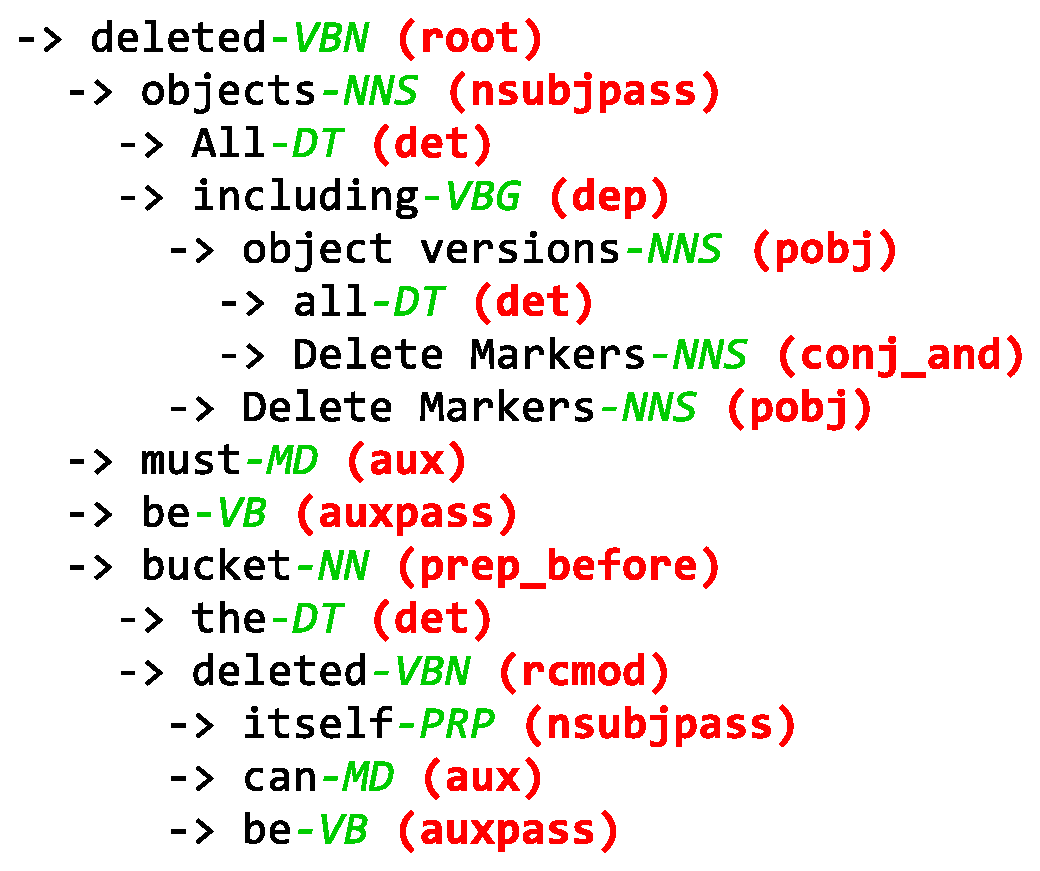
\includegraphics[scale=0.25]{StanfordAnnotated.eps}
	\caption{Sentence annotated with Stanford dependencies}
	\label{fig:standep}
\end{figure}

Next we use an example to illustrate the annotations added by the NLP Parser. Consider the sentence from the example section \textbf{\textit{`All objects (including all object versions and Delete Markers) in the bucket must be deleted before the bucket itself can be deleted.''}}. Figure~\ref{fig:standep} shows the sentence annotated by NLP parser. Each word (occurs first) is followed by the Part-Of-Speech (POS) tag of the word (in green), which is further followed by the name of Stanford dependency connecting the actual word of the sentence to its predecessor.
From an implementation perspective, this component can be implemented using any existing NLP libraries or approaches such as Stanford Parser~\cite{SNLP1}.

\subsection{Candidate Identifier}

This component accepts the annotated sentence from the previous component,
then using a trained ML model classifies whether each sentence as a temporal constraint sentence or not. We next describe the model construction.

The goal of model construction is to use a small set of manually classified temporal constraint sentences of a representative API classify the unlabeled sentences as being temporal constraints or not.
From an implementation perspective, we can use any of the standard off-the-shelf classifiers to train the ML model, since \tool\ seeks to achieve only a binary classification of the API sentences.
%For instance, model can be trained using na{\"i}ve Bayes classifier which is the simplest probabilistic classification methods and is shown to be comparative to other advanced classification methods given appropriate preprocessing~\cite{rennie2003tackling}.
The ML model can be trained offline or else by the users of the approach if better accuracy is desired for domain-specific data.

Feature selection is an important factor for the accuracy any classification method.
%For instance, na{\"i}ve Bayes classifier assumes each feature independently contributes towards the final probability of classification.
In the simplest form, each word occurring in a sentence is considered as a feature. However, such an approach may lead to overly specific ML models, and therefore the \tool\ approach extracts generic features from sentences. We next describe the features we chose for training our ML model along with the rationale for selecting such features.


1) \textbf{Length of a Sentence}: The feature is the total number of words in the sentence. The rationale is that shorter sentences (containing fewer words) are unlikely candidates for temporal constraint sentences. 

2) \textbf{Sentence Type}: The context of sentence, whether the sentence appears as method summary, parameter summary, return value summary, or exception/error summary as captured by pre-processor phase. The rationale is that a majority of the temporal constraint sentences are either summary or exception sentences. 
	
3) \textbf{Lemmatization}: The features are the lemma of a words occurring in the sentences. In linguistic, lemmatization is the reduction of operational form of a word to its base form. For instance, ``invoking'', ``invokes'', and ``invoked'' are all reduced to invoke. The rationale for reducing the words to base form is to reduce the size of the feature set that otherwise considers every word form as an independent feature. 
	
4) \textbf{Stopword Reduction}: In linguistics, stopwords are the frequently occurring words that can be ignored and are often considered noise, such as ``the'' , ``of'', ``to'' etc... The rationale for filtering the stopwords is to reduce the size of feature set that otherwise considers such words (despite being noise) as an independent features. Stopword list is further augmented by adding to them the words that occur exactly once in the training corpus to avoid over-fitting of the model to the training corpus. 
	
5) \textbf{Stanford Dependencies}: We add to the feature set by identifying the presence of specific Stanford-typed dependencies pertaining to the temporal aspects of the sentence semantics. In particular, we identify the presence of ``\textit{advcl}'', ``\textit{aux}'', ``\textit{auxpass}'', ``\textit{vmod}'', and ``\textit{tmod}''. For instance, the annotated sentence in Figure~\ref{fig:standep} contains both ``\textit{aux}'' and ``\textit{auxpass}'' dependencies. These are both added to the feature set.
	
6) \textbf{POS Tags}: We filter words whose part of speech tags are ``\textit{Noun}'', ``\textit{Determiner}'', ``\textit{Adjective}'', ``\textit{Cardinal Number}'', ``\textit{Foreign Word}'', ``\textit{Brackets}'', ``\textit{Coordinating Conjunction}'', and ``\textit{Personal Pronouns}''. The rationale for filtering based on POS tags is to remove the words that are unlikely to be specific to temporal constraints. For instance, presence or absence of determiners is unlikely to affect the outcome of classifier. We further, annotate the POS of word to further distinguish between the words used in different context.
	
7) \textbf{Sentence Structure}: The feature is the ordered sequence of chunking tags~\cite{Klein03,KleinNIPS03} in a sentence. Chunking seeks to divide a sentence into a constituent set of words (or phrases) that logically belong together (such as a Noun Phrase and Verb Phrase). Thus chunking captures the structure of a sentence. Rationale for selecting ordered sequence of chunking tags is to incorporate structure of a sentence as a feature.  
 

We use the described feature set to train a classifier to perform binary classification of sentence as either temporal constraint describing or not. The rationale of using ML based approach as opposed to a rule based approach is because: 1) rule-writing requires domain expertise; 2) rules-writing tends to quickly become ad hoc thus requires greater effort to generate generic rules to avoid over-fitting; and 3) ML classifiers have shown to scale well with large volumes of data.

 
%Constraint Extractor then classifies the sentence as a constraint 
%sentence (containing temporal constraint) candidate based on following ordered set of rules:
%
%\begin{enumerate}
%	\item The sentence is not from parameter summary or return variable summary.
%	Typically such sentences describe pre-post conditions as opposed to temporal constraints \tool\ addresses.
%	\item The sentences contains modal modifiers such as ``\textit{can, could, may, must, should}'' expressing necessity.
%	Typically, presence of such modal modifier is a strong indicator of presence of constraints imposed by an API developer
%	\item If the sentence does not contain modal modifiers described previously, sentence must contain temporal modifier relationship, identified by Stanford-typed dependency parser.
%	Typically, presence of temporal modifier is an indicator of presence of temporal information. 
%	\item If rules 2 and 3 don't apply then the sentences should be a conditional sentence, identified by the presence of keywords such as ``\textit{if}'' and ``\textit{whether}''.
%\end{enumerate}


\subsection{Text Analysis Engine}
\label{sub:TAE}

%\begin{figure}
%	\centering
%		\includegraphics[scale=0.65]{taeRep.eps}
%	\caption{First-order logic representation of annotated sentence in Figure~\ref{fig:standep}}
%	\label{fig:FOLRep}
%\end{figure}



The text analysis engine component accepts the sentences identified as constraint sentences and creates an intermediate representation of each sentence.
This intermediate representation is leveraged by subsequent component to infer formal constraints.
We define our representation as a tree structure that is mimics a FOL expression.
Research literature provides evidence of the adequacy of using FOL for NLP related analysis tasks~\cite{Sinha2009,Sinha2010,pandita12:inferring, pandita13:WHYPER}.

In our representation, every node in the tree except for the leaf nodes is a predicate node. 
The leaf nodes represent the entities.
The children of the predicate nodes are the participating entities in the relationship represented by the predicate.
The first or the only child of a predicate node is the governing entity and the second child is the dependent entity.
Together the governing entity, predicate and the dependent entity node form a tuple. 


As described in Section~\ref{sub:SENLPback} the intermediate representation generation technique is implemented as a function of Stanford-typed dependencies~\cite{Marneffe06LREC,Marneffe08COLING,KleinNIPS03}, to leverage the semantic information encoded in Stanford-typed dependencies.


However, we observed that such implementation is overwhelmed by complex sentences.
We improve the accuracy of intermediate-representation generation by proposing a hybrid approach, i.e. taking into consideration both the POS tags as well as Stanford-typed dependencies.
The POS tags which annotate the syntactical structure of a sentence are used to further simplify the constituent elements in a sentence. 
We then use the Stanford-typed dependencies that annotate the grammatical relationships between words to construct our FOL like representation.
Thus, the intermediate representation generator used in this work is a two phase process as opposed to single phase in previous work~\cite{pandita12:inferring, pandita13:WHYPER}. 
We next describe these two phases:

{\small $\bullet$} \textbf{POS Tags}: We first parse a sentence based on the function of POS tags. 
In particular, we use semantic templates to logically break a sentences into smaller constituent sentences. 
For instance, consider the sentence which are then accurately annotated by the underlying NLP Parser:

\begin{center}
\scriptsize``All objects (including all object versions and Delete Markers) in the bucket must be deleted before the bucket itself can be deleted.''. \normalsize
\end{center}

The Stanford parser faces difficulty to annotate accurately the Stanford-typed dependencies of the sentence because of presence of various clauses acting on various subject-object pairs.
As shown in Figure~\ref{fig:standep} the word including is annotated with Stanford-typed dependencies ``dep'' that is a catch all dependency. A catch all dependency is selected by a parser when no other appropriate dependency can be selected.
The \tool\ approach thus automatically break down the sentence into two smaller tractable sentences:

\begin{center}
\scriptsize \textit{``All objects in the bucket must be deleted before the bucket itself can be deleted.}''
	
\textit{``All objects including all object versions and Delete Markers.''}\normalsize 
\end{center} 


Table~\ref{tab:semanticTemplates} lists the semantic templates used in this phase.
Column ``Template'' describes conditions where the template is applicable and Column ``Summary'' describes the action taken by \tool\ when the template is applicable.
%All of these semantic templates are publicly available on our project website\footnote{\url{https://sites.google.com/site/temporalspec}}.
With respect to the previous example the template 3 \textit{(A noun phrase followed by another noun/pronoun/verb phrase in brackets)} is applicable.
Thus our shallow parser breaks the sentence into two individual sentences.
	 
\begin{table*}
\begin{center}

\caption{Semantic Templates}
    \begin{tabular}{  l  p{5cm} p{10cm} }
    \topline
    \headcol  \textbf{S No.} 	& \textbf{Template} & \textbf{Summary} \\
    \midline
    
    		1. 		& Two sentences joined by a conjunction & Sentence is broken down into two individual sentences with the conjunction term serving as the connector between two. \\
\rowcol    	2. 		& Two sentences joined by a ``,''& Sentence is broken down to individual independent sentences \\
    		3.		& A noun phrase followed by another noun/pronoun/verb phrase in brackets & Two individual sentences are formed. The first sentence is the same as the parent sentence sans the noun/pronoun.verb phrase in bracket. The second sentence constitutes of the noun phrase followed by noun/pronoun/verb phrase without the brackets.\\
\rowcol    	4.		& A noun phrase by a conditional phrase in brackets & Two individual sentences are formed. The first sentence is the same as the parent sentence sans the conditional phrase in bracket. The second sentence constitutes of noun phrases followed by conditional in the bracket.\\ 
    		5.		& A conditional phrase followed by a sentence & Two dependent sentences are formed. The first sentence constitutes the conditional phrase. The second sentence constitutes rest of the sentence.\\
\rowcol    	6.		& A sentence in which the parent verb phrase is over two child verb phrases joined by a conjunction & Two dependent sentences are formed where the dependency is the conjunction. The first sentence is formulated by removing conjunction and second child verb phrase. The second sentence is formulated by removing conjunction and first child verb phrase. \\ 
\bottomlinec
    \end{tabular}
	\label{tab:semanticTemplates}
\end{center}
\end{table*}

{\small $\bullet$} \textbf{Stanford-typed Dependencies}: After complex sentences (whenever applicable) have been broken to simple sentences, this phase generates an intermediate (FOL) representation of the sentences. This phase is equivalent to the intermediate-representation technique described in Section~\ref{sub:SENLPback}. Figure~\ref{fig:FOLTree} is the FOL representation of the sentence \textit{``All objects in the bucket must be deleted before the bucket itself can be deleted''}. All the leaf nodes (entities) are represented as the bold words. For readability each node is appended with a number representing the in-order traversal index of the tree. 

\begin{figure}
	\begin{CodeOut}
		\begin{alltt}
			01:before[6]
			02:|->must be deleted[5]
			03:\hspace*{0.2in}|->All[1]
			04:\hspace*{0.2in}|\hspace*{0.2in}|->in[3]
			05:\hspace*{0.2in}|\hspace*{0.4in}|->\textbf{objects}[2]
			06:\hspace*{0.2in}|\hspace*{0.4in}|->\textbf{bucket}[4]
			07:\hspace*{0.2in}|->can be deleted[8]
			08:\hspace*{0.4in}|->\textbf{bucket}[7]
			09:\hspace*{0.4in}|->\textbf{itself}[9]
		\end{alltt}
	\end{CodeOut}
	\caption{\label{fig:FOLTree} FOL representation of the sentence \textit{``All objects in the bucket must be deleted before the bucket itself can be deleted.''}}
\end{figure}

\subsection{Constraint Extractor}
\label{sub:ConsExtract}

Constraint Extractor is responsible for inferring temporal constraint from the classified constraint sentences.
Temporal constraints are expressed as temporal formulae involving: 
a) \textit{Predicates} $\xi$ representing method calls and 
b) \textit{Temporal operators}: backward ($\leftarrow$) \& forward ($\rightarrow$) and their negations $\xleftarrow{-}$ \& $\xrightarrow{-}$.
We define the following four constraints:

%
%
%To express temporal constraints between two methods $\xi_1,\xi_2$, there two basic constatins 
%
%\tool\ uses the formalism proposed by Lo et al.~\cite{lo2009mining} (introduced in Section~\ref{sec:background})
%for formalizing the constraints. 
%\tool\ extends the operators by proposing two additional operators:


1) \textit{Forward Operator ($\xi_1 \rightarrow \xi_2$)}: method call $\xi_1$ must be succeeded by method call $\xi_2$. 

2) \textit{Backward Operator ($\xi_1 \leftarrow \xi_2$)}: method call $\xi_1$ must be preceded by method call $\xi_2$.

3) \textit{Negative Forward Operator ($\xi_1 \xrightarrow{-} \xi_2$)}: method call $\xi_1$ cannot be succeeded by method call $\xi_2$

4) \textit{Negative Backward Operator ($\xi_1 \xleftarrow{-} \xi_2$)}: method call $\xi_1$ cannot be preceded by the method call of $\xi_2$

%The prohibition operators capture a different class of temporal constraints that cannot be
%expressed by the formulae constructed by previously proposed operators and their negations.
%For instance, the \textit{prohibition operators} seem to be negation of
%\textit{forward eventual operators} and \textit{backward eventual operators}.
%However, the negation of forward eventual operators is: not an invocation of $\xi_1$
%must be eventually followed by not an invocation of $\xi_2$. In contrast,
%\textit{prohibition operators} either negates antecedent or consequent but not both.
%In summary, we extended the formalism for temporal rules previously
%proposed by Lo et al.~\cite{lo2009mining} to express temporal constraints.

We next show how \tool\ identifies the terms of the constraint formula:


\textbf{$\xi_1$}:
\tool\ first identifies $\xi_1$ as the method whose description the constraint sentence is part of.
For instance the sentence in Figure~\ref{fig:standep} is part of Delete Bucket method description in \amazonAPI,
$\xi_1$ is instantiated as Delete Bucket method.


\textbf{$\xi_2$}:
\tool\ next identifies $\xi_2$. Since, references to $\xi_2$ may not always be implicit we leverage the semantic graphs. 
A semantic graph is a representation of objects and the methods applicable on those objects.
Figure~\ref{fig:knowledge} shows a graph for \CodeIn{Object} resource in \amazonAPI.
The phrases in rounded rectangle are the actions applicable on \CodeIn{Object} resource.
Section~\ref{sub:ACA} further describes how these graphs are generated.
%\tool\ uses the Algorithm~\ref{alg:SenAnnotaator} to identify $\xi_2$.

%\algsetup{indent=1em}
%\begin{algorithm}[t!]
%\begin{algorithmic}[1]
%\begin{scriptsize}
%\REQUIRE K\_Graph $g$, FOL\_rep $rep$ 
%\ENSURE String $action$
%\STATE $String\ action\ =\ \phi$
%\STATE $List\ r\_name\_list\ =\ g.resource\_Names$
%\STATE $FOL\_rep\ r'\ =\ rep.findLeafContaining(r\_nam\_list)$
%\STATE $List\ actionList\ =\ g.actionList$
%\WHILE{$(r'.hasParent)$}
%	\IF{$actionList.contains(r'.parent.predicate)$}
%		\STATE $action\ =\ actionList.matching(r'.parent.predicate)$
%		\STATE $break$
%	\ELSE
%		\IF{$actionList.contains(r'.leftSibling.predicate)$}
%			\STATE $action\ =\ actionList.matching(r'.leftSibling.predicate)$
%			\STATE $break$
%		\ENDIF
%	\ENDIF
%	\STATE $r'\ =\ r'.parent$
%\ENDWHILE
%\RETURN $action$
%\end{scriptsize}
%\end{algorithmic}
%\caption{Action\_Extractor}
%\label{alg:SenAnnotaator}
%\end{algorithm} 

\tool\ systematically explores the intermediate representation
of the candidate sentence to identify $\xi_2$. First, this component
attempts to locate the occurrence of object name or its synonym
in the leaf nodes (entity) of the intermediate
representation of the sentence.
Once a leaf node is found, this component systematically
traverses the tree from the leaf node to the root,
matching all parent predicates as well as immediate child
predicates.
This component matches each of the traversed predicate
with the actions associated with the object defined in
semantic graph. 
\tool\ further employs WordNet and Lemmatisation to deal with
synonyms to find appropriate matches. If a match is
found, then the matching action is returned as $\xi_2$.
\tool\ does not consider self references, that is if $\xi_2 = \xi_1$, the identified method reference is discarded.
In case of multiple matching actions \tool\ considers only the first match.
For instance the sentence in Figure~\ref{fig:standep} algorithm identifies
Delete Object method as $\xi_2$

\textbf{Temporal Operator}:
\tool\ next identifies the direction (forward or backward) of the relationship by examining the tense of $\xi_2$ reference in the sentence.
Past tense is considered as backward and other tenses are considered as forward.
For instance, the sentence in Figure~\ref{fig:standep} since ``deleted'' is in past tense and therefore operator is backward and the constraint is 
Delete Bucket $\leftarrow$ Delete Object.

The negation is identified by presence of the negation verbs such as ``\textit{no}'', ``\textit{not}'', ``\textit{can't}'' ... etc.
Another rule for negation operator is if the sentence is in exception/error description. 



\subsection{Semantic-Graph Generator}
\label{sub:ACA}

A key way of identifying reference to a method in the API by \tool\ is the employment of a semantic graph of an API.
We propose to initially infer such graphs from API documents.
Ad hoc creation of semantic graph is prohibitively time consuming and may be error prone.
We thus employ a systematic methodology (proposed previously in Whyper ~\cite{pandita13:WHYPER}) to infer semantic graphs from API documents.

We first consider the name of the class for the API document in question.
We then find the synonyms terms used refer to the class in question.
The synonym terms are listed as by splitting the camel-case notation in the class name.
This list is further augmented with the name of the parent classes and implemented interfaces if any. We then systematically inspect the member methods to identify actions applicable to the objects represented by the class. From the name of a public method (describing a possible action on the object), we extract verb phrases. The verb phrases are used as the associated actions applicable on the object. In case of REST API we first identified the resources and then listed REST actions on those resources as applicable actions. Figure~\ref{fig:knowledge} shows the graph for \CodeIn{Object} resource in REST API. The phrases in rounded rectangle are the REST actions applicable on \CodeIn{Object} resource in \amazonAPI.

\begin{figure}
	\centering
	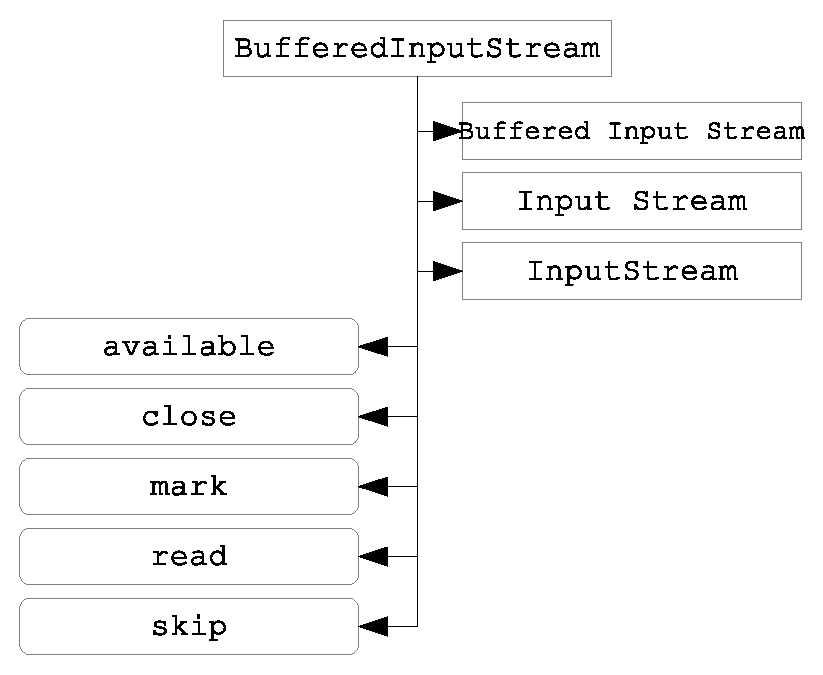
\includegraphics[scale=0.3]{KnowledgeGraph.eps}
	\caption{Semantic Graph for the \CodeIn{Object} related operations in Amazon S3 REST API}
	\label{fig:knowledge}
\end{figure}

\subsection{Type Analysis}
\label{sub:typeAnalysis}

Some temporal constraints are enforced by the type system in typed Languages.
For instance, a method ($m$) accepting input parameter ($i$) of type ($t$) mandates that (at least one) method ($m'$) be invoked whose return value is of type ($t$).
To extend the temporal constraints inferred by the analyzing the natural language text, this component infers additional constraints that are encoded
in the type system. %Algorithm~\ref{alg:TypeAnalysis} lists the steps followed to infer type based temporal constraints.

%The algorithm accepts the list of methods as an input produces a graph with
%the nodes representing methods in an API and the directed edges representing temporal constraints.
First, an index list ($L_{mtd}$) of the public methods in an API is created based on the return types of the method.
Next, all public methods in the API are added as nodes ($m_1,m_2...m_k$) in an unconnected graph ($G$).
Next, for every method ($m$) in $L_{mtd}$, we identify the types
of the input parameters ($t_1,t_2...t_k$).
We then add a directed edge from all the methods in ($G$), where the return type of the method matches any of the types in ($t_1,t_2...t_k$). 
Additionally, an edge is created from the object creation methods (constructors) of a class to the non-static members methods of a class, because a member methods are invoked after objects creation. 
The temporal constraints based on the type information is extracted by querying $G$. 
The incoming edges to a node denoting a method represents the set of pre-requisite methods.
The temporal constraint being, at least one of the pre-requisite methods must be invoked before invoking the method in question.


%\begin{algorithm}[t!]
%\begin{algorithmic}[1]
%\begin{scriptsize}
%\REQUIRE List $methodList$ 
%\ENSURE Graph $seq\_Graph$
%\STATE $Graph\ seq\_Graph\ =\ \phi$
%\STATE $Map\ idx\ = createIdx(methodList)$
%
%\FORALL{$Method\ mtd\ in\ methodList$} 
%	\STATE $seq\_Graph.addVertex(mtd)$
%\ENDFOR
%
%\FORALL{$Method\ mtd\ in\ methodList$} 
%	\IF{$mtd.isPublic()$}
%		\IF{$!mtd.isStatic()$}
%			\STATE $List\ preList\ =\ idx.query(mtd.declaringType)$
%			\FORALL{$Method\ mtd'\ in\ preList$}
%				\STATE $seq\_Graph.addEdge(mtd',mtd)$
%			\ENDFOR
%		\ENDIF
%		\FORALL{$Parameter\ param\ in\ mtd.getParameters()$}
%			\IF{$!isBasicType(param.Type)$}
%				\STATE $List\ preList\ =\ idx.query(paramType)$
%				\FORALL{$Method\ mtd'\ in\ preList$}
%					\STATE $seq\_Graph.addEdge(mtd',mtd)$
%				\ENDFOR				
%			\ENDIF
%		\ENDFOR
%	\ENDIF
%\ENDFOR
%\RETURN $seq\_Graph$
%\end{scriptsize}
%\end{algorithmic}
%\caption{Type\_Sequence\_Builder}
%\label{alg:TypeAnalysis}
%\end{algorithm} 

